\section{Opening, reopening, and market boundaries}
\label{sec:opening}

An opening calculation acts on a collection of accumulated eligible orders. It does not have the same event sequence as a stream of continuous aggressors. Nor does a futures market have a universal cash-equity-style closing auction. Opening, session termination, daily settlement, and final expiry must each have their own transition.

\subsection{Eligible quantities and candidate prices}

Fix a finite candidate grid $\mathcal P$ and a snapshot of auction-eligible simple orders. Define
\begin{equation}
 B(p)=\sum_{i\in\mathcal B}q_i\ind\{L_i\ge p\},\qquad
 S(p)=\sum_{i\in\mathcal S}q_i\ind\{L_i\le p\}.
\end{equation}
Under complete one-for-one compatibility,
\begin{equation}
 V(p)=\min\{B(p),S(p)\},\qquad I(p)=B(p)-S(p).
\label{eq:auction}
\end{equation}
The function $B$ is nonincreasing, $S$ is nondecreasing, and $I$ is nonincreasing. An executable opening can contain a crossed book during accumulation because continuous matching is not active in that phase. The same crossed ledger would not be an ordinary stable continuous book.

\begin{proposition}[Auction capacity under full compatibility]
At a fixed $p$, the maximum feasible match quantity is $V(p)$.
\end{proposition}
\begin{proof}
Every trade consumes one eligible contract on each side, giving the upper bound $\min(B,S)$. Pair contracts from the two sides until the smaller side is exhausted. Full compatibility makes every pair admissible, so the bound is attained.
\end{proof}

Account restrictions, minimum quantities, ratio instruments, and other incompatibilities can invalidate this construction. In such cases $V(p)$ should be defined through feasible matching rather than assumed equal to a minimum of totals.

\subsection{CME opening-price branches}

CME's IOP documentation begins with maximum matching quantity. Its rules and worked applications then distinguish imbalance and reference-price cases: minimum unmatched quantity, upward selection for buy-side pressure, downward selection for sell-side pressure, and proximity to prior settlement for a balanced interval \citep{CMEIOPRules,CMEIOPExamples}. We implement the following documented simple-order cases, preserving any unresolved tie as a set rather than inventing a final preference.

Let $\mathcal P_0=\argmax_pV(p)$. If it is a singleton, the primary criterion suffices. For multiple candidates, the examples establish selection of a unique minimum of $|I(p)|$ when one exists, including a zero-versus-nonzero tie in volume. When the maximum-volume candidates all have positive imbalance, choose the highest such price; when all have negative imbalance, choose the lowest. When all are balanced, choose the candidate nearest prior settlement; equal distances remain set-valued here. A remaining two-sided exact tie requires further product and operational treatment beyond these examples.

These branches are compatible with the monotonicity of $I$. On an all-positive candidate set, the highest price has the smallest imbalance; on an all-negative set, the lowest price does. This observation explains the direction of the pressure rule without assuming that every tie is resolved by a generic reference-distance minimization.

\begin{table}[htbp]
\centering\small
\begin{tabular}{@{}lrrrr@{}}
\toprule
Candidate price & $B(p)$ & $S(p)$ & $V(p)$ & $I(p)$\\
\midrule
100 & 15 & 4 & 4 & 11\\
101 & 15 & 9 & 9 & 6\\
102 & 10 & 12 & 10 & $-2$\\
103 & 6 & 12 & 6 & $-6$\\
\bottomrule
\end{tabular}
\caption{A synthetic opening ledger. Buy limits are $103:6$, $102:4$, $101:5$; sell limits are $100:4$, $101:5$, $102:3$. Notation $p:q$ denotes price and contracts.}
\label{tab:opening}
\end{table}

The unique price in Table~\ref{tab:opening} is 102. With a declared price-time allocation on both sides, the two highest-priced buys fill six and four contracts. The sells fill four at limit 100, five at limit 101, and one at limit 102. All ten pairs execute at the selected opening price 102; their limits are eligibility conditions rather than distinct execution prices.

\begin{figure}[htbp]
\centering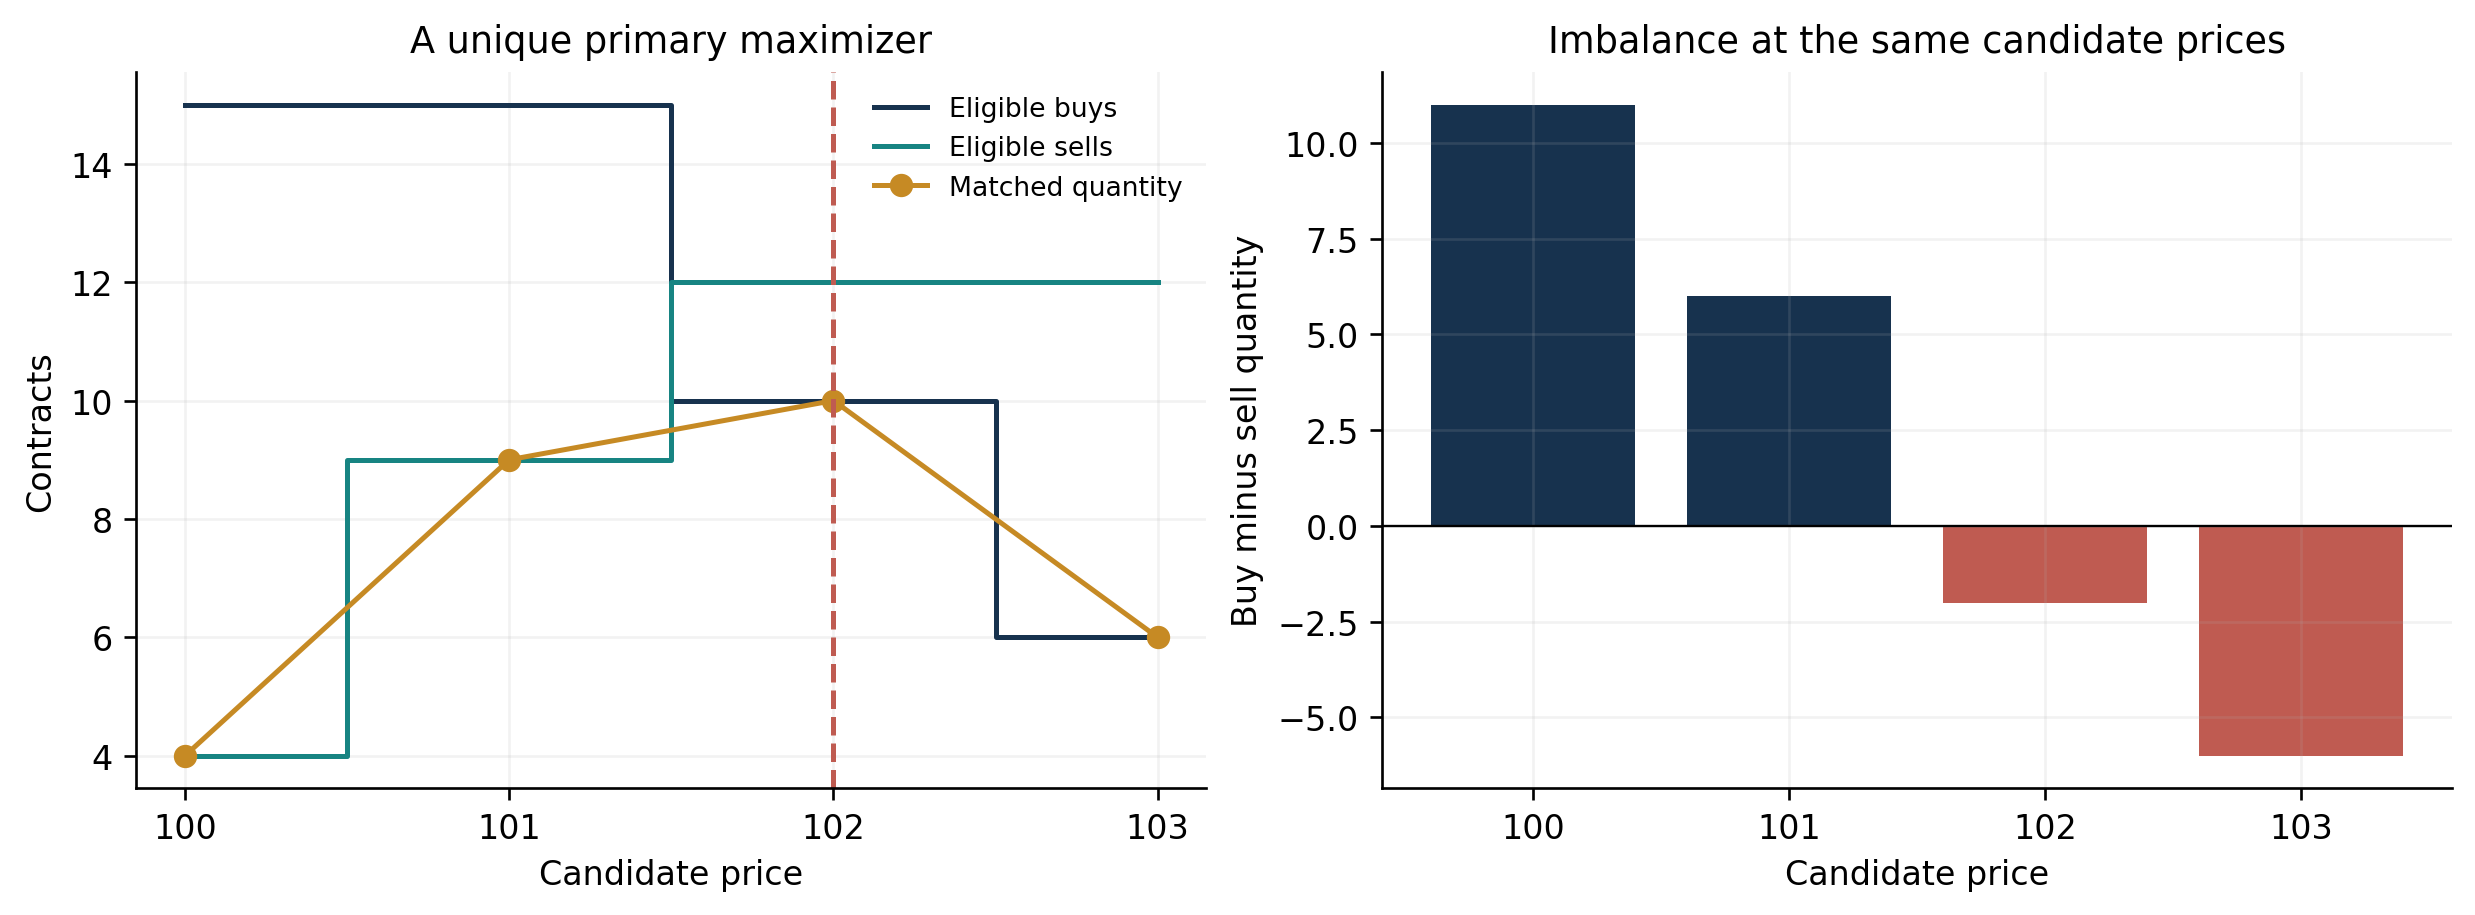
\includegraphics[width=\textwidth]{figures/05_opening.png}
\caption{The quantity and imbalance calculations for Table~\ref{tab:opening}. Price 102 has the largest match quantity despite a sell imbalance. Maximizing volume and setting imbalance to zero are different objectives.}
\label{fig:opening}
\end{figure}

\begin{table}[htbp]
\centering\small
\begin{tabularx}{\textwidth}{@{}lXXXl@{}}
\toprule
Case & Buy orders & Sell orders & Maximizing prices & IOP\\
\midrule
Buy pressure & $103:6$ & $101:4$ & $101,102,103$ & 103\\
Sell pressure & $103:4$ & $101:6$ & $101,102,103$ & 101\\
Balanced & $103:4$ & $101:4$ & $101,102,103$ & 102\\
Opposite signs & $102:4,101:2$ & $101:4,102:3$ & $101,102$ & 101\\
Zero and positive & $102:4,101:2$ & $101:4$ & $101,102$ & 102\\
\bottomrule
\end{tabularx}
\caption{Five synthetic tie cases, with reference settlement 102. The opposite-sign case has imbalances $2$ and $-3$; the last case has imbalances $2$ and $0$. Candidate prices are the listed integer ticks.}
\label{tab:ties}
\end{table}

Opening allocation must be specified separately from opening-price selection. For example, CME's SOFR documentation describes price-time opening treatment, with TOP matching beginning in continuous trading and implied interest unavailable in pre-open \citep{CMEMatching}. One should not apply a continuous-session proportional allocator automatically to an opening ledger.

\subsection{Stop election as a finite activation process}

The IOP rules describe recalculation when an indicative price elects stop orders, using their limit-price quantities until no additional stops are elected \citep{CMEIOPRules}. An abstract implementation starts from an active set $E_0$, calculates $p(E_0)$, and repeatedly applies
\begin{equation}
 E_{k+1}=E_k\cup\{i:\text{stop }i\text{ is elected by }p(E_k)\}.
\end{equation}

\begin{proposition}[Finite activation closure]
If there are $N$ initially inactive stops, no new orders arrive during the calculation, and an elected stop remains active, the iteration has at most $N$ strict enlargements before reaching a fixed active set.
\end{proposition}
\begin{proof}
The active sets form an increasing chain of subsets of a finite set. Every strict enlargement adds at least one previously inactive stop. There can be at most $N$ such additions.
\end{proof}

The proof does not establish that indicative prices are monotone. It also does not resolve an ambiguous price-selection branch. A reproducible algorithm needs both a fixed activation convention and a price-selection rule defined for its inputs. The supplied numerical opening examples contain no stops, so they do not depend on a hidden convention for unresolved ties.

\subsection{A primary-volume stability margin}

\begin{proposition}[A sharp functional gap bound]\label{prop:gap}
Suppose $V$ on a finite grid has a unique maximizer $p^*$ and gap
\begin{equation}
 g=V(p^*)-\max_{p\ne p^*}V(p)>0.
\end{equation}
If $\|\widehat V-V\|_\infty\le\varepsilon$ and $g>2\varepsilon$, then $p^*$ remains the unique primary maximizer. The constant two is sharp over arbitrary bounded perturbations of $V$.
\end{proposition}
\begin{proof}
For any competitor $p$, $\widehat V(p^*)-\widehat V(p)\ge g-2\varepsilon>0$. For sharpness choose a runner-up $p_2$, lower $V(p^*)$ by $\varepsilon$, and raise $V(p_2)$ by $\varepsilon$. The resulting difference is $g-2\varepsilon$, giving a tie at equality and reversal below it.
\end{proof}

If both cumulative sides change by at most $\delta$ uniformly, then $|\min(\widehat B,\widehat S)-\min(B,S)|\le\delta$, so the same sufficient bound applies with $\varepsilon=\delta$. The sharpness construction is a statement about the class of volume functions; it need not be realizable by a single order amendment in a constrained book. In Table~\ref{tab:opening}, the volume gap is only one contract, illustrating the limited protection afforded by the primary criterion alone.

\subsection{Closing a session and controlling prices}

For a phase boundary, let $\mathcal P(\phi)$ be the permitted price set and $\mathcal E(\phi)$ the permitted events. A resting order outside a new permitted range is not automatically a trade. An execution transition must also have a compatible counterparty and a matching phase. Clipping a simulated transaction price to a limit while keeping its quantity is therefore generally incorrect.

In the ES rulebook, trading-day termination is distinct from the afternoon reference interval used for price controls; the ordinary session extends beyond that interval \citep{CME358}. Our model treats session close as a phase transition with order-lifetime processing. Section~\ref{sec:settlement} separately treats the daily settlement statistic. Neither operation is assumed to be a uniform-price closing auction.
\FloatBarrier
